\chapter{Fractals and chaos}
\label{ch:fractals}

The United States Geological Survey (USGS) hosts a
catalog\footnote{\href{https://earthquake.usgs.gov/earthquakes/search/}{\tt
    https://earthquake.usgs.gov/earthquakes/search/}} of global
earthquakes. Here is a histogram of the 20,000 most recent earthquakes
with magnitude 4.5 or greater, which was downloaded when this text was
written.

\noindent\begin{minipage}[t][][b]{.4\textwidth}
  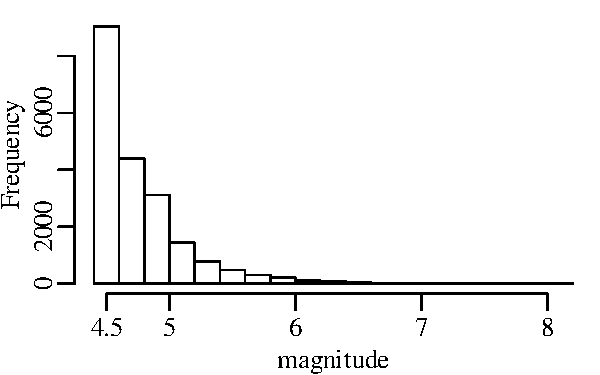
\includegraphics[width=\textwidth]{../figures/recentquakes.pdf}\medskip
\end{minipage}
\begin{minipage}[t][][t]{.6\textwidth}
  \captionof{figure}{Histogram for 20,000 recent earthquakes of
    magnitude $\geq{4.5}$ from the USGS earthquake catalog.}
  \label{fig:recentquakes}
\end{minipage}

This distribution is positively skewed (section~\ref{sec:shape}), and
therefore has a similar appearance as the clast size distribution of
Figure~\ref{fig:negativeKDE}. Recall that the skewness of the clast
size distribution caused the mean and the median to be very different
(Figure~\ref{fig:clastslocation}). This problem was solved by a simple
logarithmic transformation (Figure~\ref{fig:logKDE}). After taking
logs, the skewed distribution of clast sizes became symmetric
(section~\ref{sec:transformations}).  In fact, we could apply a
$\chi^2$- or Kolmogorov-Smirnov test to show that the log of the clast
sizes follows a normal distribution.  This type of skewed
distribution, which becomes normal after taking logarithms, is called
a \textbf{lognormal} distribution. Let's see if this procedure also
works for the earthquake data:\medskip

\noindent\begin{minipage}[t][][b]{.4\textwidth}
  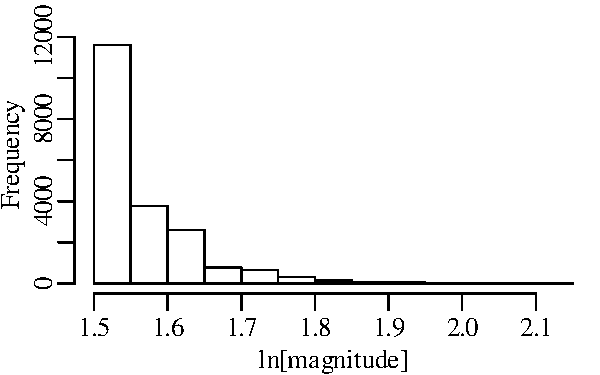
\includegraphics[width=\textwidth]{../figures/recentlogquakes.pdf}\medskip
\end{minipage}
\begin{minipage}[t][][t]{.6\textwidth}
  \captionof{figure}{ The histogram of the logarithm of the 20,000
    earthquakes in Figure~\ref{fig:recentquakes} is still positively
    skewed.}
  \label{fig:recentlogquakes}
\end{minipage}

The logarithmic transformation has not reduced the skewness of the
data. This means that the earthquake magnitudes do not follow a
lognormal distribution. And it also means that logarithms cannot fix
the discrepancy between the mean and the median. In fact the
distribution of earthquake magnitudes \emph{does not have a
  well-defined mean or median}. This phenomenon is very common in
geology.

\section{Power law distributions}
\label{sec:power-law}

In our attempt to remove the skewness of the earthquake magnitude
data, we ignored the fact that earthquake magnitudes are already a
logarithmic quantity, which can take negative values. In fact we will
see that most seismic events have negative magnitudes!  So instead of
taking the logarithm of the earthquake magnitudes, let us take the
logarithm of the frequencies:

\noindent\begin{minipage}[t][][b]{.3\textwidth}
  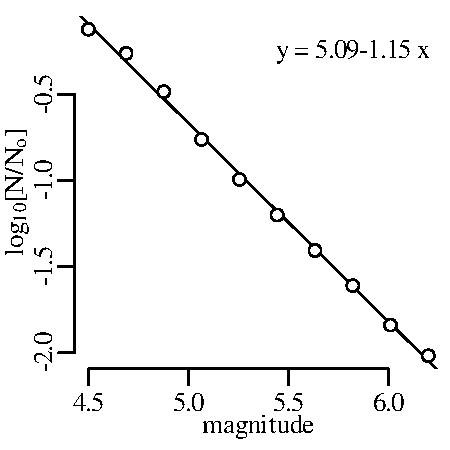
\includegraphics[width=\textwidth]{../figures/gutenberg.pdf}\medskip
\end{minipage}
\begin{minipage}[t][][t]{.7\textwidth}
  \captionof{figure}{ Bivariate scatter plot of
    $y=\log_{10}[N/N_\circ]$ against earthquake magnitude, where $N$
    is the number of earthquakes exceeding a given magnitude and
    $N_\circ$ is the total number of earthquakes, which is 20,000 for
    the dataset of Figure~\ref{fig:recentquakes}.
 }
  \label{fig:gutenberg}
\end{minipage}

The transformed data plot on a straight line of the form
\begin{equation}
  \log_{10}[N/N_\circ] = a + b~\mbox{magnitude}
  \label{eq:gutenberg}
\end{equation}

\noindent where $a = 5.09$ and $b =
-1.15$. Equation~\ref{eq:gutenberg} is called the
\textbf{Gutenberg-Richter Law} and is a mainstay of seismology. It is
tremendously useful for predictive purposes. Given a record of small
seismic events, the Gutenberg-Richter Law allows accurate predictions
of seismic hazards posed by larger events. For example, given that the
20,000 earthquakes of Figure~\ref{fig:recentquakes} span a continuous
period of 1031 days, we can use Equation~\ref{eq:gutenberg} to predict
the likelihood that an earthquake of magnitude 9.0 or greater will
happen within the next year:

\begin{enumerate}
\item The expected number of earthquakes per year is
  \[
  \frac{20000\mbox{~earthquakes}}{1031\mbox{~days}}\times{365}\mbox{~days}
  = 7080 \mbox{~earthquakes}
  \]

\item Plugging magnitude 9.0 into Equation~\ref{eq:gutenberg}:
  \[
  \log_{10}[N/N_\circ] = 5.09 -1.15~\times{9.0} = -5.26
  \]

\item Rearranging for $N$:
  \[
  N = 7080 \times 10^{-5.26} = 0.039
  \]
\end{enumerate}

In other words, there is a 3.9\% chance that at least one magnitude
earthquake 9.0 or greater earthquake happens per year. This is
equivalent to 1 such event occurring per 25~years, or 4 events
occurring per century. If we look at the last magnitude $\geq{9.0}$
earthquakes of the past century:

\begin{center}
  \begin{tabular}{c|ccccc}
    location & Japan & Sumatra & Alaska & Chile & Kamchatka \\
    year & 2011 & 2004 & 1964 & 1960 & 1952 \\
    magnitude & 9.1 & 9.2 & 9.2 & 9.5 & 9.0
  \end{tabular}
\end{center}

\noindent then that amounts to 5 events. This seems to indicate that
the short term earthquake record can indeed be used to make long term
predictions.\medskip

Power-law relationships are found in many other geoscience fields. For
example, in hydrology:

\noindent\begin{minipage}[t][][b]{.3\textwidth}
  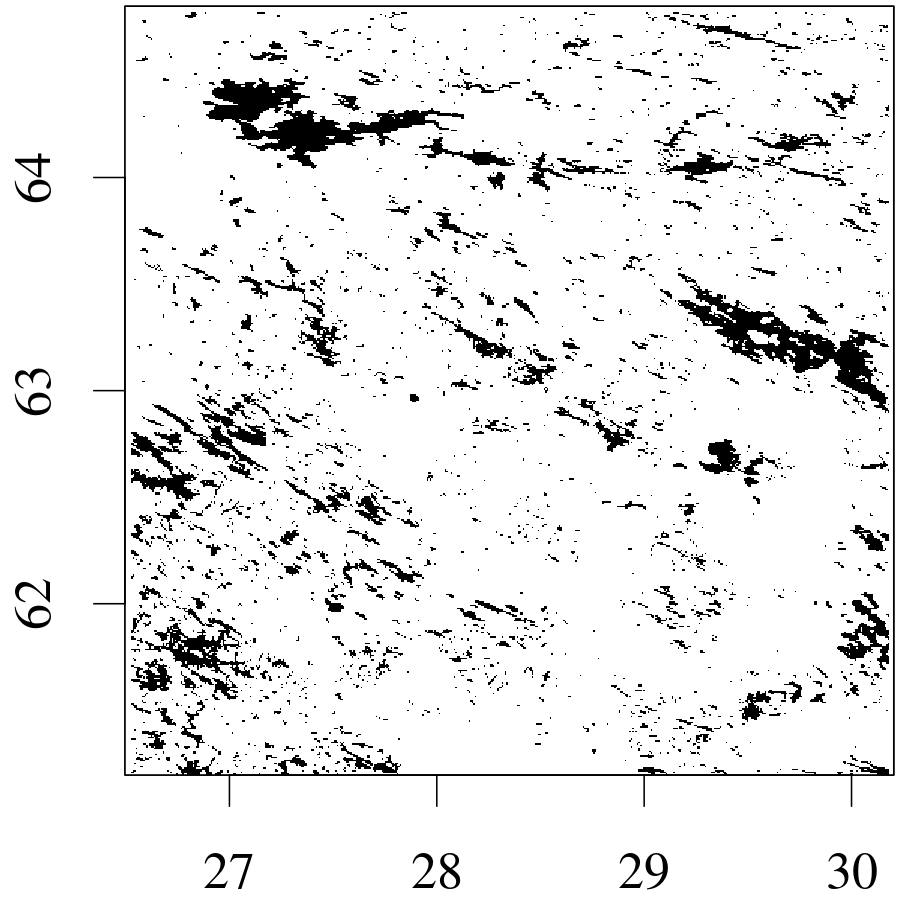
\includegraphics[width=\textwidth]{../figures/Finland.png}
\end{minipage}
\begin{minipage}[t][][t]{.7\textwidth}
  \captionof{figure}{A map of central Finland (axis labels mark
    latitude and longitude), with water marked in black and land
    marked in white. Finland is also known as ``the land of a thousand
    lakes''. But in fact there are far more than 1000 lakes in
    Finland.  The small area shown in this figure already contains
    2327 of them. Most of these lakes are small, but there are also a
    few big ones that cover an area of more than
    1000~km\textsuperscript{2}.}
  \label{fig:Finland}
\end{minipage}

The size-frequency relationship of Finnish lakes looks very similar to
the Gutenberg-Richter Law of earthquakes:

\noindent\begin{minipage}[t][][b]{.3\textwidth}
  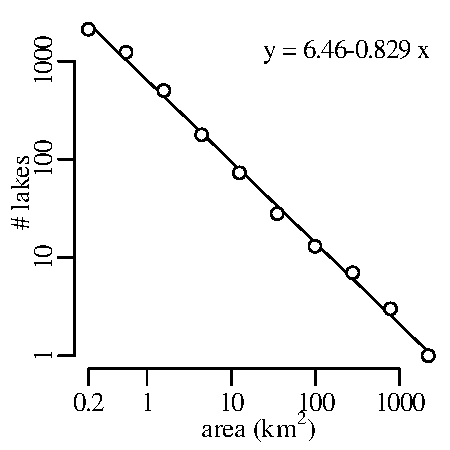
\includegraphics[width=\textwidth]{../figures/Finland.pdf}
\end{minipage}
\begin{minipage}[t][][t]{.7\textwidth}
  \captionof{figure}{Plotting the number of lakes exceeding a certain
    size against that size on a log-log scale yields a linear array of
    points similar to the Gutenberg-Richter Law of
    Figure~\ref{fig:gutenberg}. Extrapolating this trend towards the
    left would reveal that there are millions of puddles in Finland.}
  \label{fig:Finlandpowerlaw}
\end{minipage}

Other examples of similar power law relationships in the Earth
Sciences include the size-frequency distributions of faults and
joints, clasts in glacial till, oil fields and ore deposits, rivers
and their tributaries, mountains and floods, to name just a few.

\section{How long is the coast of Britain?}
\label{sec:britain}

In a famous paper\footnote{Mandelbrot, B., 1967. How long is the coast
  of Britain? Statistical self-similarity and fractional
  dimension. \textit{Science}, 156(3775), pp.636-638.}, Benoit
Mandelbrot showed that it is impossible to unequivocally pin down the
circumference of Britain. The answer depends on the length of the
measuring rod:\medskip

\noindent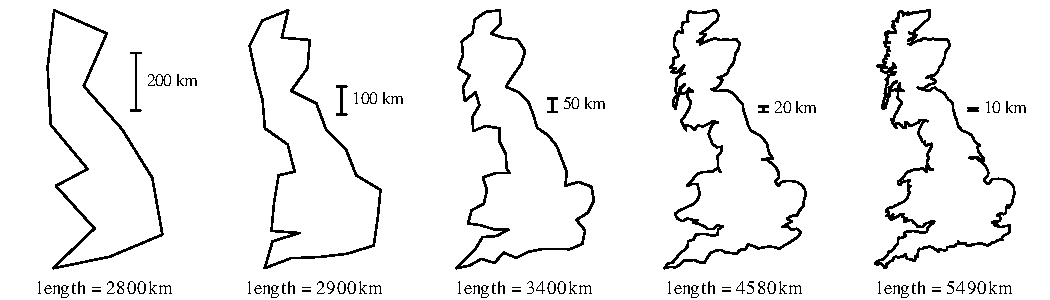
\includegraphics[width=\textwidth]{../figures/britain.pdf}
\begingroup
\captionof{figure}{Five attempts to measure the length of
  Britain's coastline. Different results are obtained depending on the
  length of the measuring rod used for the measurements. The shorter
the yardstick (shown as error bars), the longer the estimate.\medskip}
\endgroup

However this seemingly complex phenomenon can be fully captured by a
simple \textbf{power law} equation. Plotting the length of the coastline
against the size of the measuring rod on a log-log scale:

\noindent\begin{minipage}[t][][b]{.3\textwidth}
  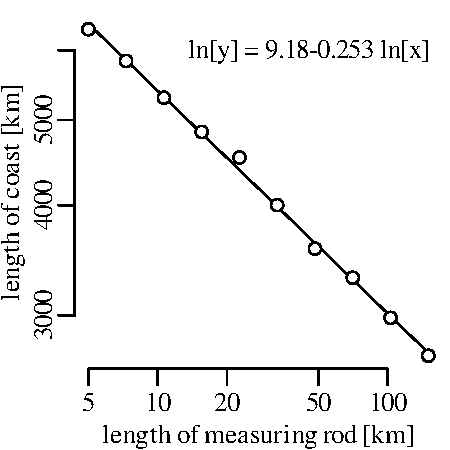
\includegraphics[width=\textwidth]{../figures/loglogbritain.pdf}\medskip
\end{minipage}
\begin{minipage}[t][][t]{.7\textwidth}
  \captionof{figure}{Setting out the length of the British coast line
    against the length of the measuring rod on a log-log scale
    produces a linear trend with a slope of $-0.253\pm{0.018}$ (95\%
    confidence). This line can be extrapolated to lower values to
    estimate the length that would be measured with even smaller
    measuring rods. For example, if we were to measure the British
    coast with a 30~cm long ruler, then this would produce a result of
    $\exp(9.18-0.253\ln[3\times{10}^{-4}])=42,060$~km!  }
  \label{fig:loglogbritain}
\end{minipage}

An alternative (and equivalent) way to plot the data is to divide the
measured length of the coastline by the length of the measuring rod to
obtain the number of linear segments that approximate the British
coast.  Plotting this number against the length of the measuring rod
on a log-log plot also produces a straight line:

\noindent\begin{minipage}[t][][b]{.3\textwidth}
  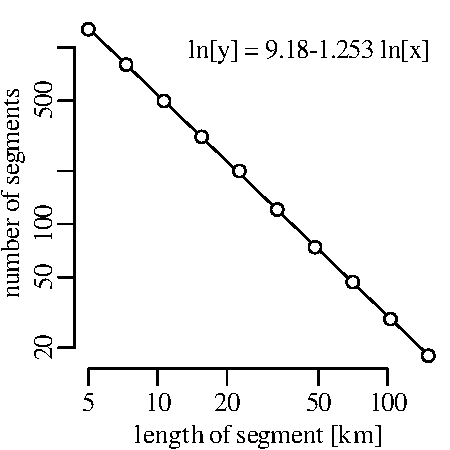
\includegraphics[width=\textwidth]{../figures/fractaldimbritain.pdf}\medskip
\end{minipage}
\begin{minipage}[t][][t]{.7\textwidth}
  \captionof{figure}{The same data as Figure~\ref{fig:loglogbritain}
    but plotting the number of polygonal segments on the y-axis
    instead of the length of those segments. Note how the slope of the
    best fit line equals the slope of Figure~\ref{fig:loglogbritain}
    minus one.}
  \label{fig:fractaldimbritain}
\end{minipage}

\textbf{Box counting} is another way to obtain this result. Instead of
approximating the British coast with a set of line segments, this
method covers the coast with a set of boxes. Varying the box size and
counting the number of boxes needed to cover the entire coast:\medskip

\noindent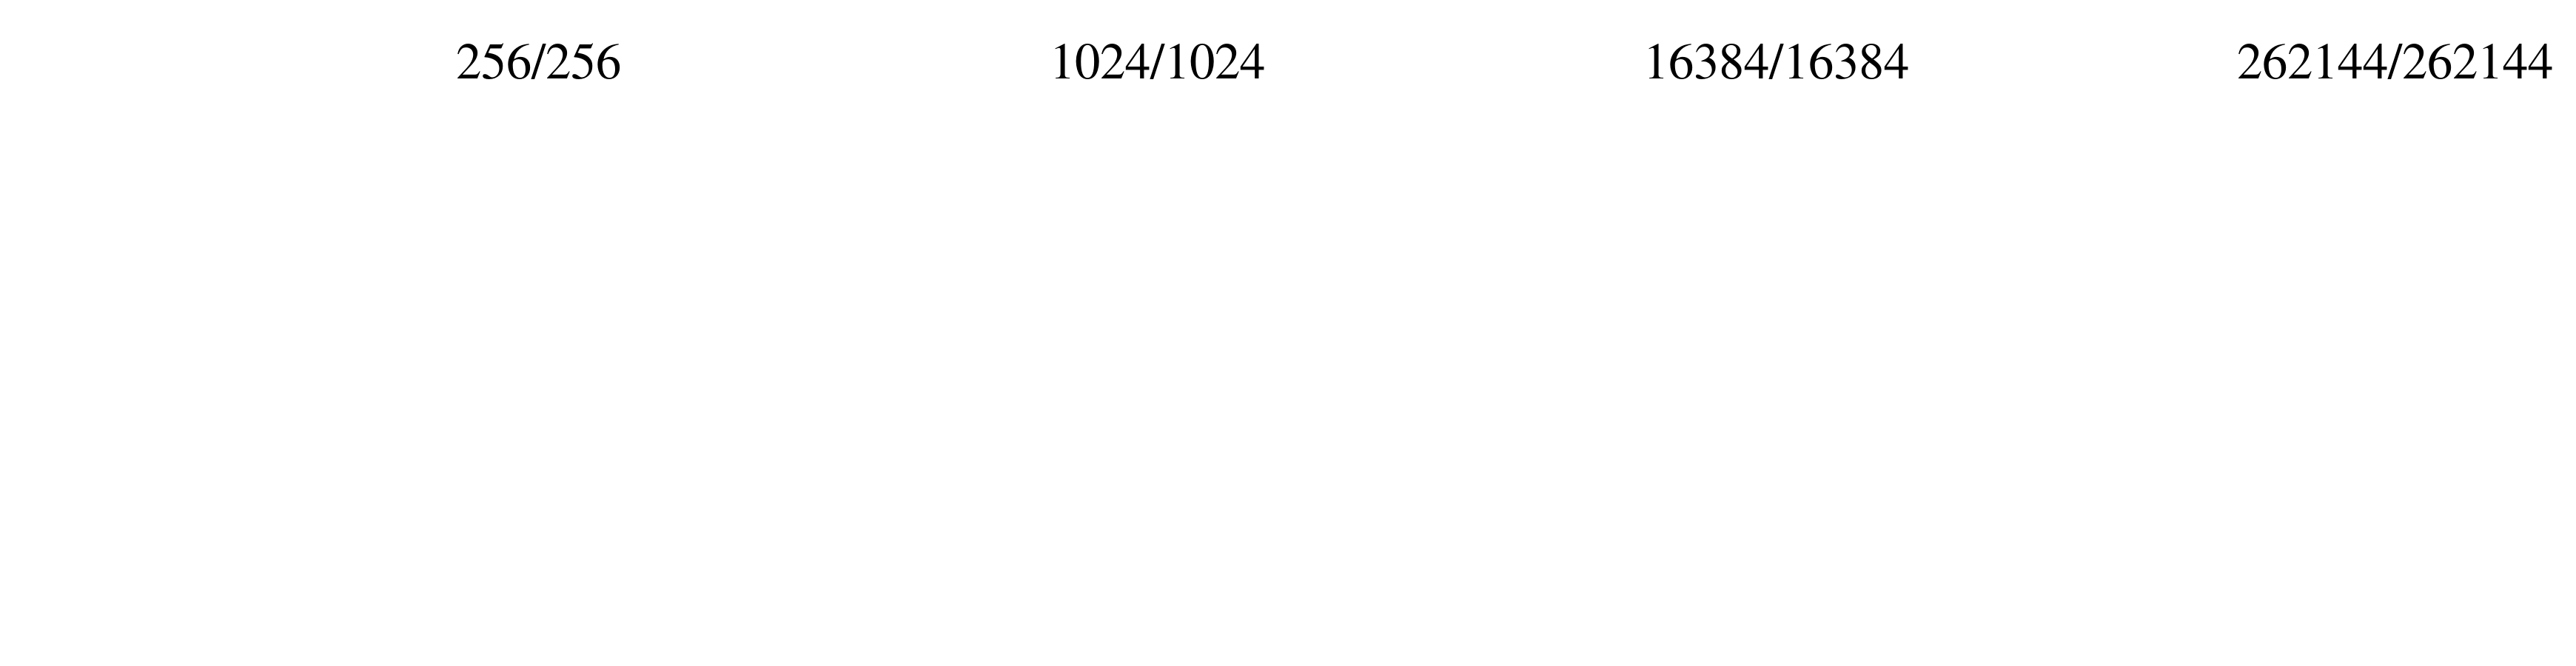
\includegraphics[width=\textwidth]{../figures/Britainboxes.png}
\begingroup \captionof{figure}{Box counting of the British coast using
  (from left to right) a $16\times{16}$, $32\times{32}$,
  $64\times{64}$, and $128\times{128}$ grid. Black squares overlap
  with the coastline, white squares do not. The legends in the upper
  right corner of each subpanel specify the number of black squares
  relative to the total number of squares.\medskip}
  \label{fig:Britainboxes}
\endgroup

Instead of plotting the number of line segments against their size, we
plot the number of boxes against their size (width). This produces a
linear trend that has a different intercept than
Figure~\ref{fig:Britainboxes}, but a similar slope:\medskip

\noindent\begin{minipage}[t][][b]{.3\textwidth}
  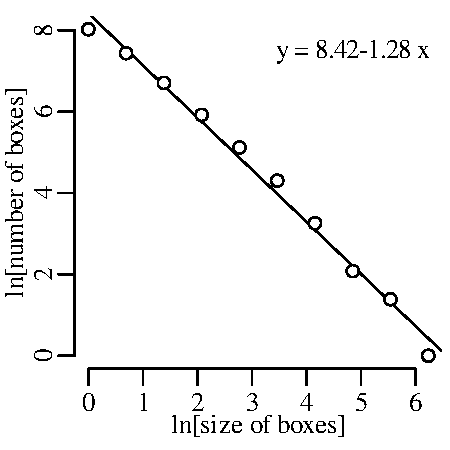
\includegraphics[width=\textwidth]{../figures/Britainboxcounts.pdf}\medskip
\end{minipage}
\begin{minipage}[t][][t]{.7\textwidth}
  \captionof{figure}{Plotting the number of boxes against their size
    on a log-log diagram yields a linear array with a slope of
    $-1.28\pm{0.10}$.  This is similar to the value obtained by the
    polygonal line segment method of
    Figure~\ref{fig:fractaldimbritain}.  }
  \label{fig:Britainboxcounts}
\end{minipage}

The box counting method is more flexible, and therefore more widely
used, than the line segment method. For example, applying the same
technique to a river network:\medskip

\noindent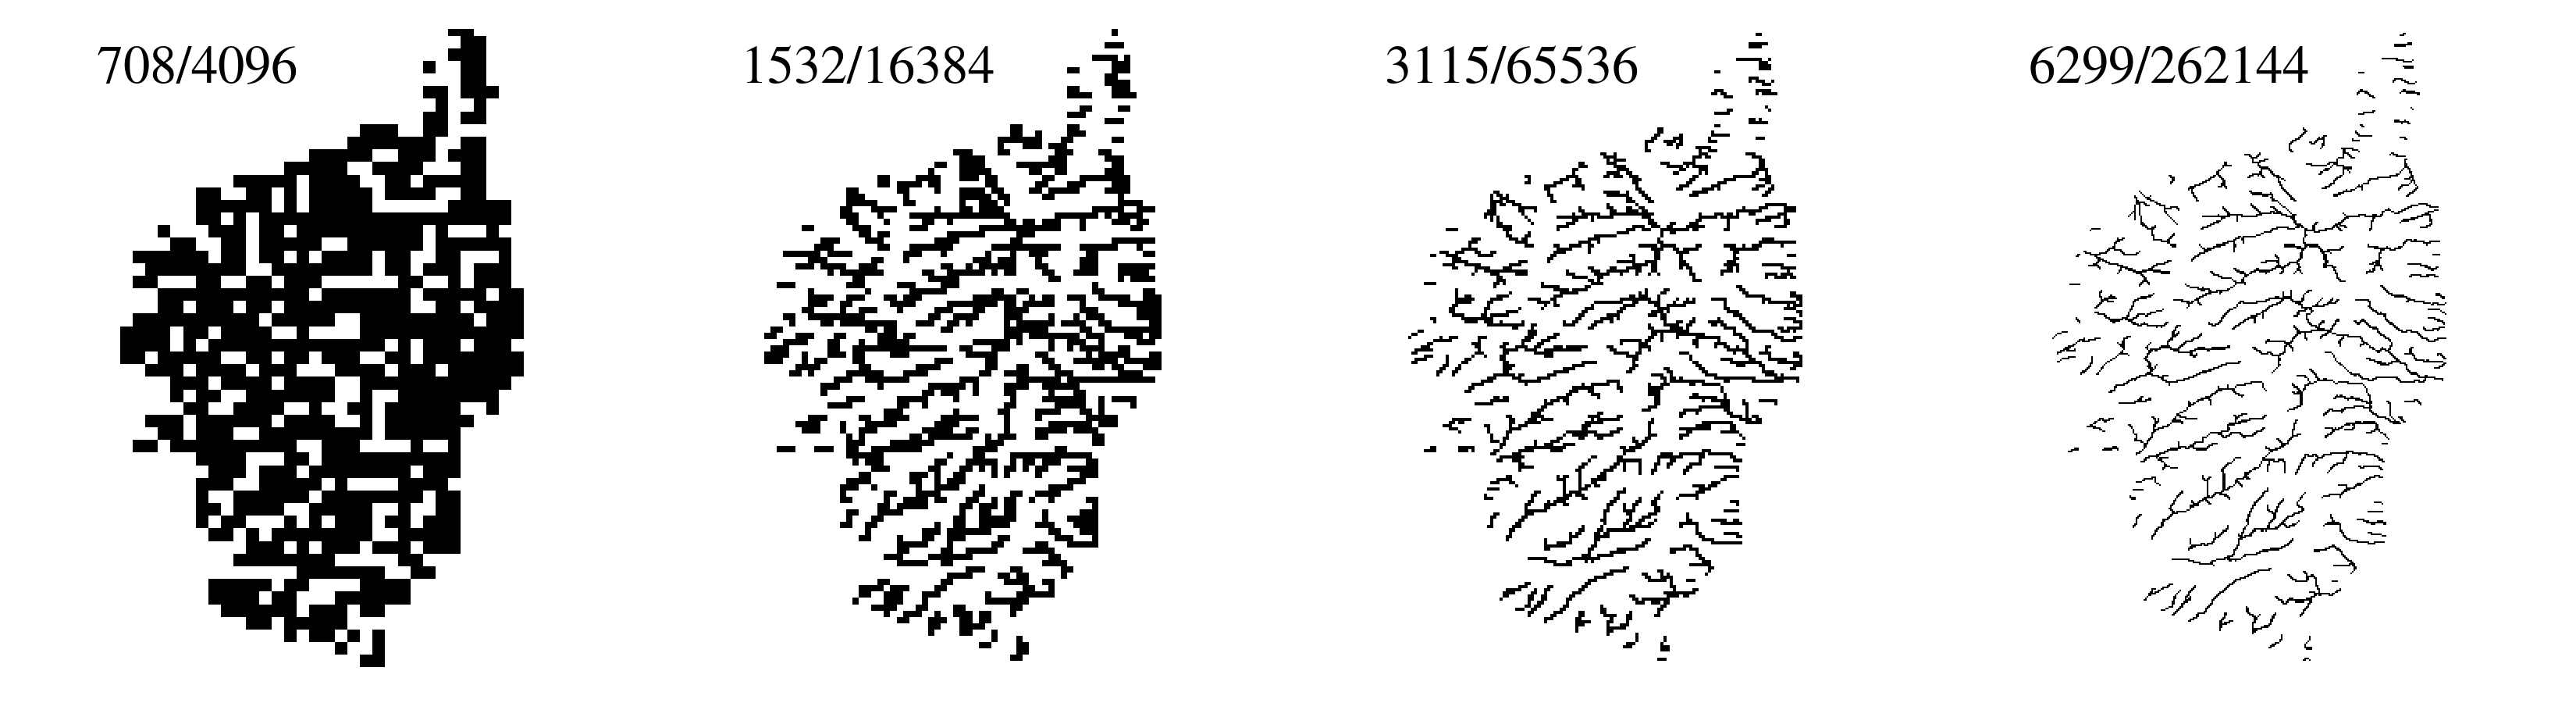
\includegraphics[width=\textwidth]{../figures/Corsica.png}
\begingroup \captionof{figure}{Box counting of the river network on
  the island of Corsica (France). Black boxes overlap with rivers,
  white boxes do not.  Legends are as in
  Figure~\ref{fig:Britainboxes}.\medskip}
\label{fig:Corsica}
\endgroup

\noindent and visualising the results on a log-log plot:

\noindent\begin{minipage}[t][][b]{.3\textwidth}
  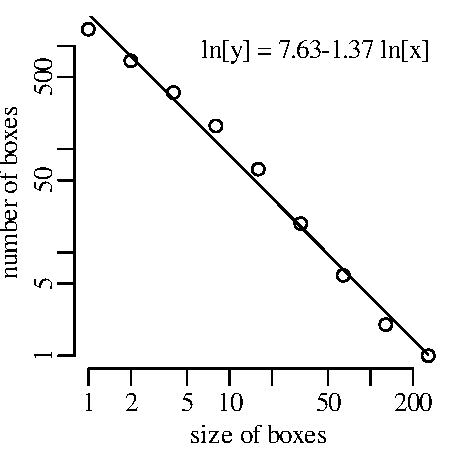
\includegraphics[width=\textwidth]{../figures/Corsicaboxcounts.pdf}\medskip
\end{minipage}
\begin{minipage}[t][][t]{.7\textwidth}
  \captionof{figure}{Log-log plot of the box counting results of
    Figure~\ref{fig:Corsica}. The power law appears to be a law of
    nature.  }
  \label{fig:Corsicaboxcounts}
\end{minipage}

\section{Fractals}
\label{sec:fractals}

This section will introduce some simple geometric patterns that match
the statistical properties of geological patterns such as the
coastlines, lakes and river networks of section~\ref{sec:britain}.
The first of these synthetic patterns is the \textbf{Koch curve},
which is created by a simple \textbf{recursive algorithm}.

\noindent\begin{minipage}[t][][b]{.5\textwidth}
  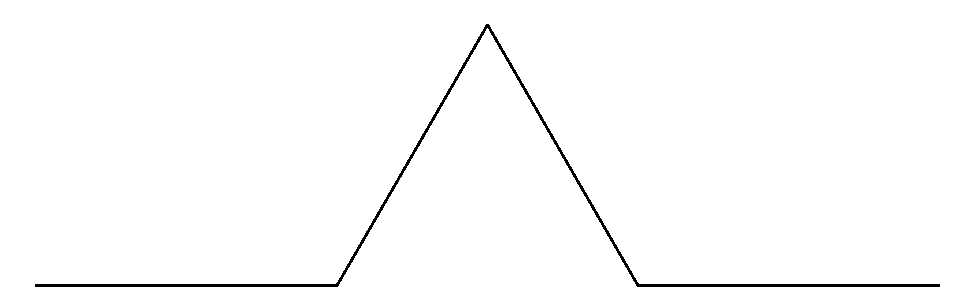
\includegraphics[width=\textwidth]{../figures/koch1.pdf}\medskip
\end{minipage}
\begin{minipage}[t][][t]{.5\textwidth}
  \captionof{figure}{A 1\textsuperscript{st} order Koch curve is
    constructed by (1) dividing a straight line segment into three
    segments of equal length; (2) drawing an equilateral triangle that
    has the middle segment from step 1 as its base and points outward;
    and (3) removing the line segment that is the base of the triangle
    from step 2.  }
  \label{fig:koch1}
\end{minipage}

\noindent\begin{minipage}[t][][b]{.5\textwidth}
  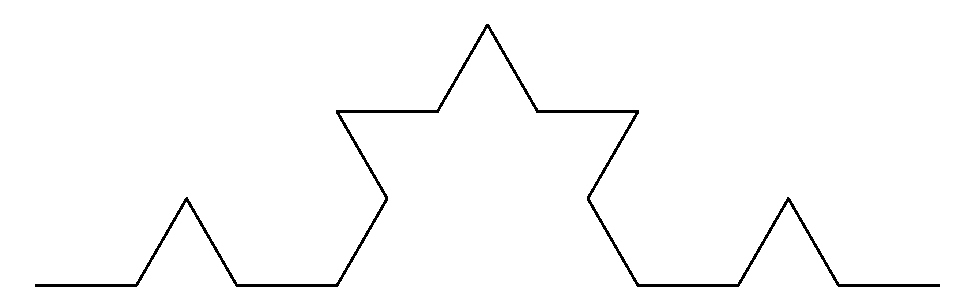
\includegraphics[width=\textwidth]{../figures/koch2.pdf}\medskip
\end{minipage}
\begin{minipage}[t][][t]{.5\textwidth}
  \captionof{figure}{A 2\textsuperscript{nd} order Koch curve is
    derived from a 1\textsuperscript{st} order Koch curve by replacing
    each straight line segment in the 1\textsuperscript{st} order
    curve with a scaled down version of that 1\textsuperscript{st}
    order curve.}
  \label{fig:koch2}
\end{minipage}

\noindent\begin{minipage}[t][][b]{.5\textwidth}
  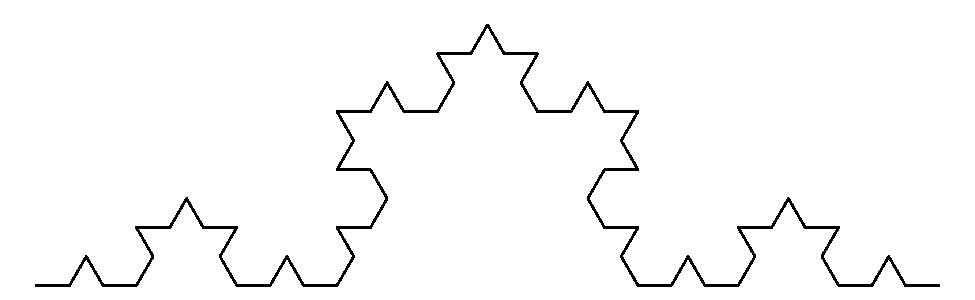
\includegraphics[width=\textwidth]{../figures/koch3.pdf}\medskip
\end{minipage}
\begin{minipage}[t][][t]{.5\textwidth}
  \captionof{figure}{A 3\textsuperscript{rd} order Koch curve is
    derived from a 2\textsuperscript{nd} order Koch curve by replacing
    each straight line segment in the 2\textsuperscript{nd} order
    curve with a scaled down version of the 1\textsuperscript{st}
    order Koch curve.}
  \label{fig:koch3}
\end{minipage}

\noindent\begin{minipage}[t][][b]{.5\textwidth}
  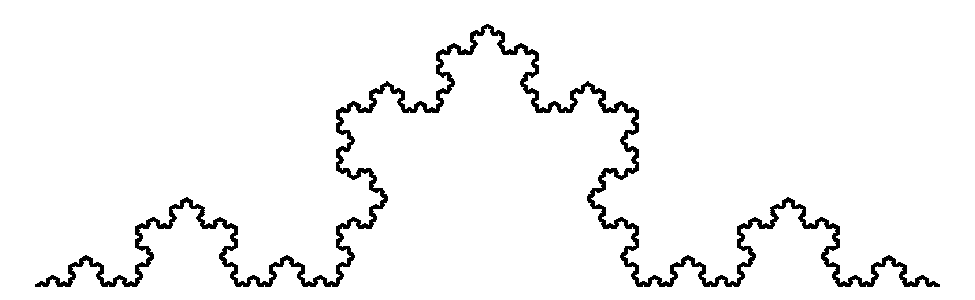
\includegraphics[width=\textwidth]{../figures/koch6.pdf}\medskip
\end{minipage}
\begin{minipage}[t][][t]{.5\textwidth}
  \captionof{figure}{This is a 6\textsuperscript{th} order Koch curve,
    which is generated by replacing each straight line segment in a
    5\textsuperscript{th} order curve with a scaled down version of
    the 1\textsuperscript{st} order curve.}
  \label{fig:koch6}
\end{minipage}

This procedure can be repeated \emph{ad infinitum}, producing an
intricate curve that is endlessly detailed. It is similar in many ways
to the British coast line, which also produces ever more detail as we
zoom into the map. Measuring the length of a Koch curve presents the
same difficulty as measuring the length of the British coastline: the
answer depends on the length of the measuring rod. Applying the box
counting method to the Koch curve:\medskip

\noindent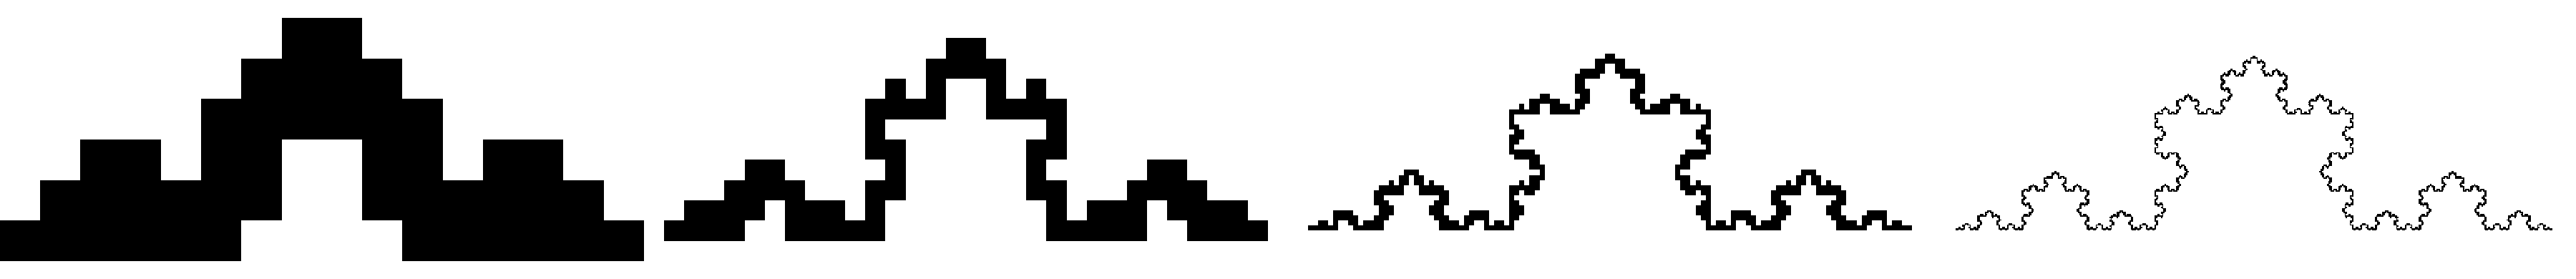
\includegraphics[width=\textwidth]{../figures/koch.png}
\begingroup \captionof{figure}{Box counting of the
  6\textsuperscript{th} order Koch curve. The larger the boxes, the
  fewer of them are needed to cover the entire curve. The recursive
  order of the Koch curve can be increased indefinitely, and so does
  the number of small boxes needed to cover them.\medskip}
\label{fig:kochboxes}
\endgroup

Plotting the results on a frequency-magnitude log-log plot:

\noindent\begin{minipage}[t][][b]{.3\textwidth}
  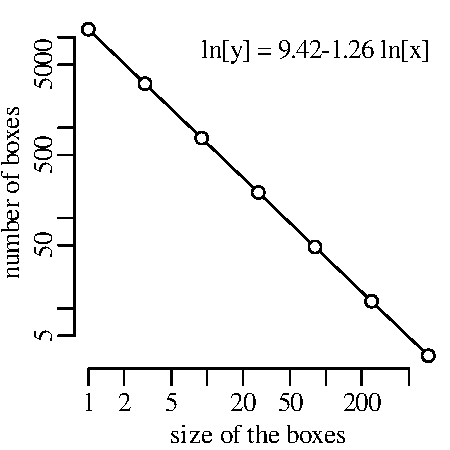
\includegraphics[width=\textwidth]{../figures/kochboxcounts.pdf}\medskip
\end{minipage}
\begin{minipage}[t][][t]{.7\textwidth}
  \captionof{figure}{Log-log plot setting out the number of boxes
    needed to cover the 6\textsuperscript{th} order Koch curve of
    Figure~\ref{fig:koch6} against the size of those boxes.  The best
    fitting line has a slope of $-1.21\pm{0.07}$, which is similar to
    the slope of the box-counting results for the British coastline
    (Figure~\ref{fig:Britainboxcounts}).  }
  \label{fig:kochboxcounts}
\end{minipage}

The similarity of Figures~\ref{fig:Britainboxcounts} and
\ref{fig:kochboxcounts} suggest that the Koch curve serves as an
\emph{artificial coastline}. The Koch curve is just one of many
artificial fractals. Here is another one:\medskip

\noindent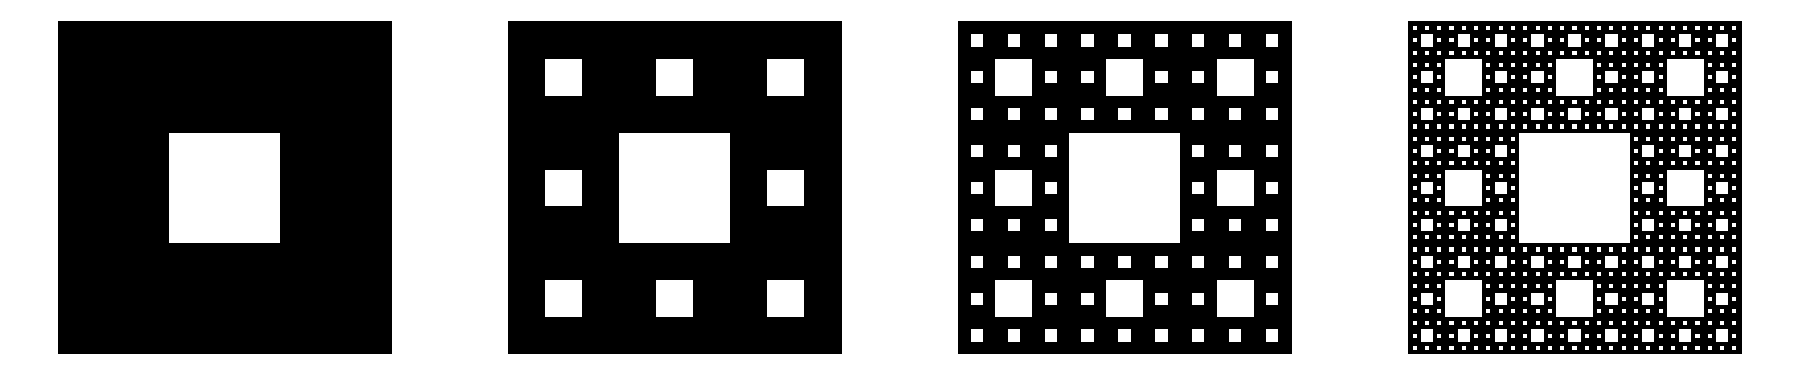
\includegraphics[width=\textwidth]{../figures/sierpinski.pdf}
\begingroup \captionof{figure}{The \textbf{Sierpinski carpet} is
  generated using a recursive algorithm that is built on a grid of
  eight black squares surrounding a white square. Each level of
  recursion replaces each black square by the same pattern. From left
  to right, this figure shows the first four levels of recursion for
  this algorithm. The end result is an arrangement of small and large
  holes that shares many characteristics with the size distribution of
  Finnish lakes shown in Figure~\ref{fig:Finland}.\medskip }
\label{fig:sierpinski}
\endgroup

One thing that the Koch curve and Sierpinski carpet have in common
is their \textbf{self-similarity}. Their level of complexity remains
the same regardless of scale. Whether one zooms in or out of the picture,
the complexity remains the same.\medskip

Because it consists of boxes, the Sierpinski carpet is ideally suited
for box counting. We can either cover the black areas with boxes, or
do the same with the white areas. Here is the resulting log-log
plot:\medskip

\noindent\begin{minipage}[t][][b]{.3\textwidth}
  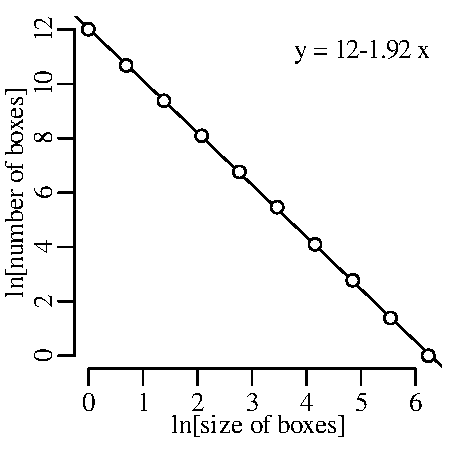
\includegraphics[width=\textwidth]{../figures/sierpinskiboxcounts.pdf}\medskip
\end{minipage}
\begin{minipage}[t][][t]{.7\textwidth}
  \captionof{figure}{Log-log plot of the box counting results for the
    Sierpinski carpet. This pattern in ideally suited for box
    counting, resulting in a perfect linear fit. Note how the slope of
    the best fitting line ($-1.92\pm{0.02}$) is greater than that of
    the Koch curve (Figure~\ref{fig:kochboxcounts}). It is similar to
    the slope that would be obtained by box-counting the Finnish lakes
    of Figure~\ref{fig:Finland}, which similar to $x-1$ where $x$ is
    the slope of the size-frequency plot of the Finnish lakes
    (Figure~\ref{fig:Finlandpowerlaw}).}
  \label{fig:sierpinskiboxcounts}
\end{minipage}

Mathematically, the linear fit of the log-log plots can written as
\begin{equation}
  \ln[\mbox{number of boxes}] = C - D \times \ln[\mbox{size of boxes}]
  \label{eq:fractaldim}
\end{equation}

The slope magnitude of the line ($D$) is also known as the
\textbf{fractal dimension} of the pattern. It is called a
\emph{dimension} because it has all the characteristics of the spatial
dimensions, which can be used to chacterise a point ($D=0$), a line
($D=1$), a plane ($D=2$) or a cube ($D=3$). But whereas these
traditional notions of dimension are tied to integer numbers, the
dimensionality of fractals is quantified by a non-integer
\emph{fraction}. Formalising the box-counting procedure leads to an
alternative definition of the fractal dimension:
\begin{equation}
  D = -\lim\limits_{\epsilon \to 0}\frac{\ln{N(\epsilon)}}{\ln{\epsilon}}
  \label{eq:Minkowski}
\end{equation}

\noindent where $\epsilon$ is the size of the box and $N(\epsilon)$ is
the number of boxes needed to cover the feature of
interest. Equation~\ref{eq:Minkowski} can be used to obtain exact
analytical expressions for deterministic fractals. Thus, it can be
shown that the fractal dimension of a Koch curve is
$D=\log_{3}(4)=1.262$. This is a number between $D=1$ (a line) and
$D=2$ (a plane). It reflects the intricate curvature of the Koch
curve, which partly `fills' the 2-dimensional plane.  The Sierpinski
carpet has a fractal dimension of $D=\log_{3}(8)=1.893$. This number,
too, falls between the dimensionalities of a line and a plane. But it
is more similar to a plane than it is to a line.\medskip

Other shapes exist that have fractal dimensions between $0 < D < 1$ or
between $2 < D < 3$. Consider, for example, the \textbf{Cantor set}:

\noindent\begin{minipage}[t][][b]{.4\textwidth}
  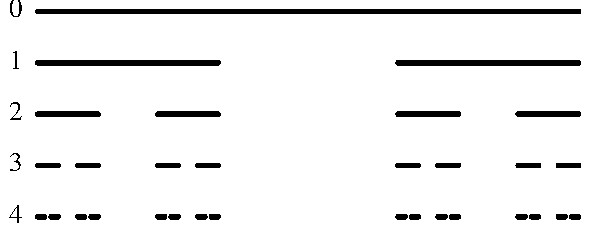
\includegraphics[width=\textwidth]{../figures/cantor.pdf}\medskip
\end{minipage}
\begin{minipage}[t][][t]{.6\textwidth}
  \captionof{figure}{The Cantor set is generated using a recursive
    algorithm that is built on a line segment whose middle third is
    removed. Each level of recursion replaces each black line by the
    same pattern. From top to bottom, this figure shows the first five
    levels of recursion for this algorithm. }
  \label{fig:cantor}
\end{minipage}

Plotting the size distribution of the Cantor set on a log-log scale:

\noindent\begin{minipage}[t][][b]{.3\textwidth}
  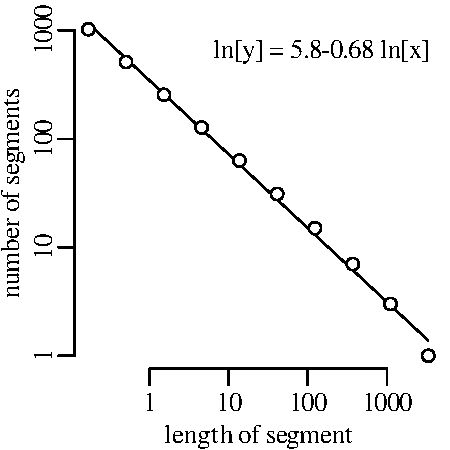
\includegraphics[width=\textwidth]{../figures/cantorloglog.pdf}\medskip
\end{minipage}
\begin{minipage}[t][][t]{.7\textwidth}
  \captionof{figure}{The y-axis shows the number of linear segments in
    the Cantor set that exceed the length shown on the x-axis. The
    values form a power law with a fractal dimension of
    $D=0.64\pm{0.01}$.  Using Equation~\ref{eq:Minkowski}, it can be
    shown that the exact value is $D=\ln[2]/\ln[3]=0.631$. With a
    fractal dimension between zero and one, the Cantor set falls
    somewhere between a point and a line.}
  \label{fig:cantorloglog}
\end{minipage}

\section{Chaos}
\label{sec:chaos}

Consider the following experimental setup:

\noindent\begin{minipage}[t][][b]{.4\textwidth}
  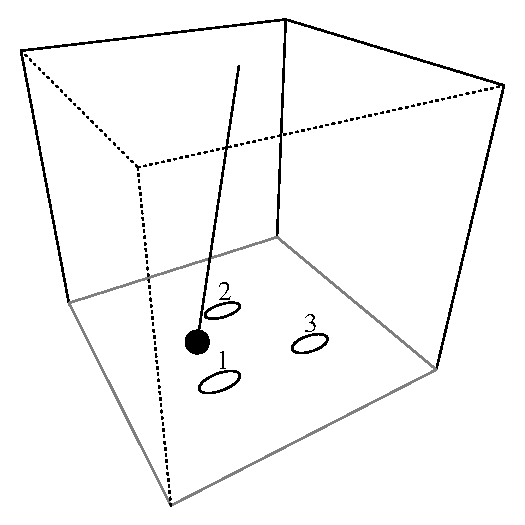
\includegraphics[width=\textwidth]{../figures/pendulum.pdf}\medskip
\end{minipage}
\begin{minipage}[t][][t]{.6\textwidth}
  \captionof{figure}{A pendulum is swinging above three magnets. The
    force ($F_m$) exerted on the pendulum scales with the square of
    its bob's distance ($|d|$) to the magnets ($F_m(i) \propto
    1/|d(i)|^2$, where $1\leq{i}\leq{3}$ marks each of the magnets).
    The pendulum slows down due to friction ($F_f(i) \propto v$ where
    $v$ is the velocity of the bob) and eventually comes to a
    standstill above one of the magnets. On this figure it has done so
    above the first magnet.}
  \label{fig:pendulum}
\end{minipage}

Despite the simplicity of this setup, it can lead to some complex
behaviour.

\noindent\begin{minipage}[t][][b]{.33\textwidth}
  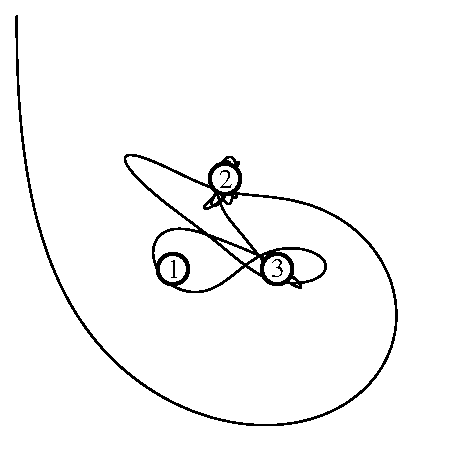
\includegraphics[width=\textwidth]{../figures/3magnets1.pdf}\medskip
\end{minipage}
\begin{minipage}[t][][t]{.67\textwidth}
  \captionof{figure}{This figure shows the three magnet configuration
    of Figure~\ref{fig:pendulum} in map view. The black line marks the
    trajectory of the pendulum after it was pushed southward from a
    position towards the northwest of the three magnets.  After
    describing a circular motion, the bob of the pendulum accelerates
    towards the second magnet, gets deflected by it, and slows down.
    It then heads towards the third magnet and the first magnet before
    returning to the second magnet and coming to a standstill there.
  }
  \label{fig:3magnets1}
\end{minipage}

Moving the initial position of the bob slightly to the south of the
previous position results in a different outcome:

\noindent\begin{minipage}[t][][b]{.33\textwidth}
  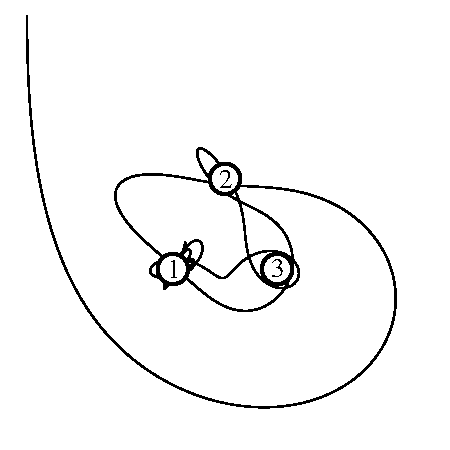
\includegraphics[width=\textwidth]{../figures/3magnets2.pdf}\medskip
\end{minipage}
\begin{minipage}[t][][t]{.67\textwidth}
  \captionof{figure}{The experimental setup shown in this figure is
    nearly identical to that of Figure~\ref{fig:3magnets1}. The only
    difference is a slight offset of the initial position. The first
    stage of the resulting trajectory is nearly identical to that of
    Figure~\ref{fig:3magnets1}. The bob makes a circular motion
    towards the second magnet and decelerates. But after passing the
    second magnet, its course diverges from the first experiment. It
    moves towards the first magnet, to the third magnet and then back
    to the first magnet before coming to a standstill. Thus, the
    slight difference in initial position has produced a completely
    different end result.}
  \label{fig:3magnets2}
\end{minipage}

We can repeat the experiment for any other initial
position. Evaluating the outcomes along a $512\times{512}$ grid of
initial values:

\noindent\begin{minipage}[t][][b]{.4\textwidth}
  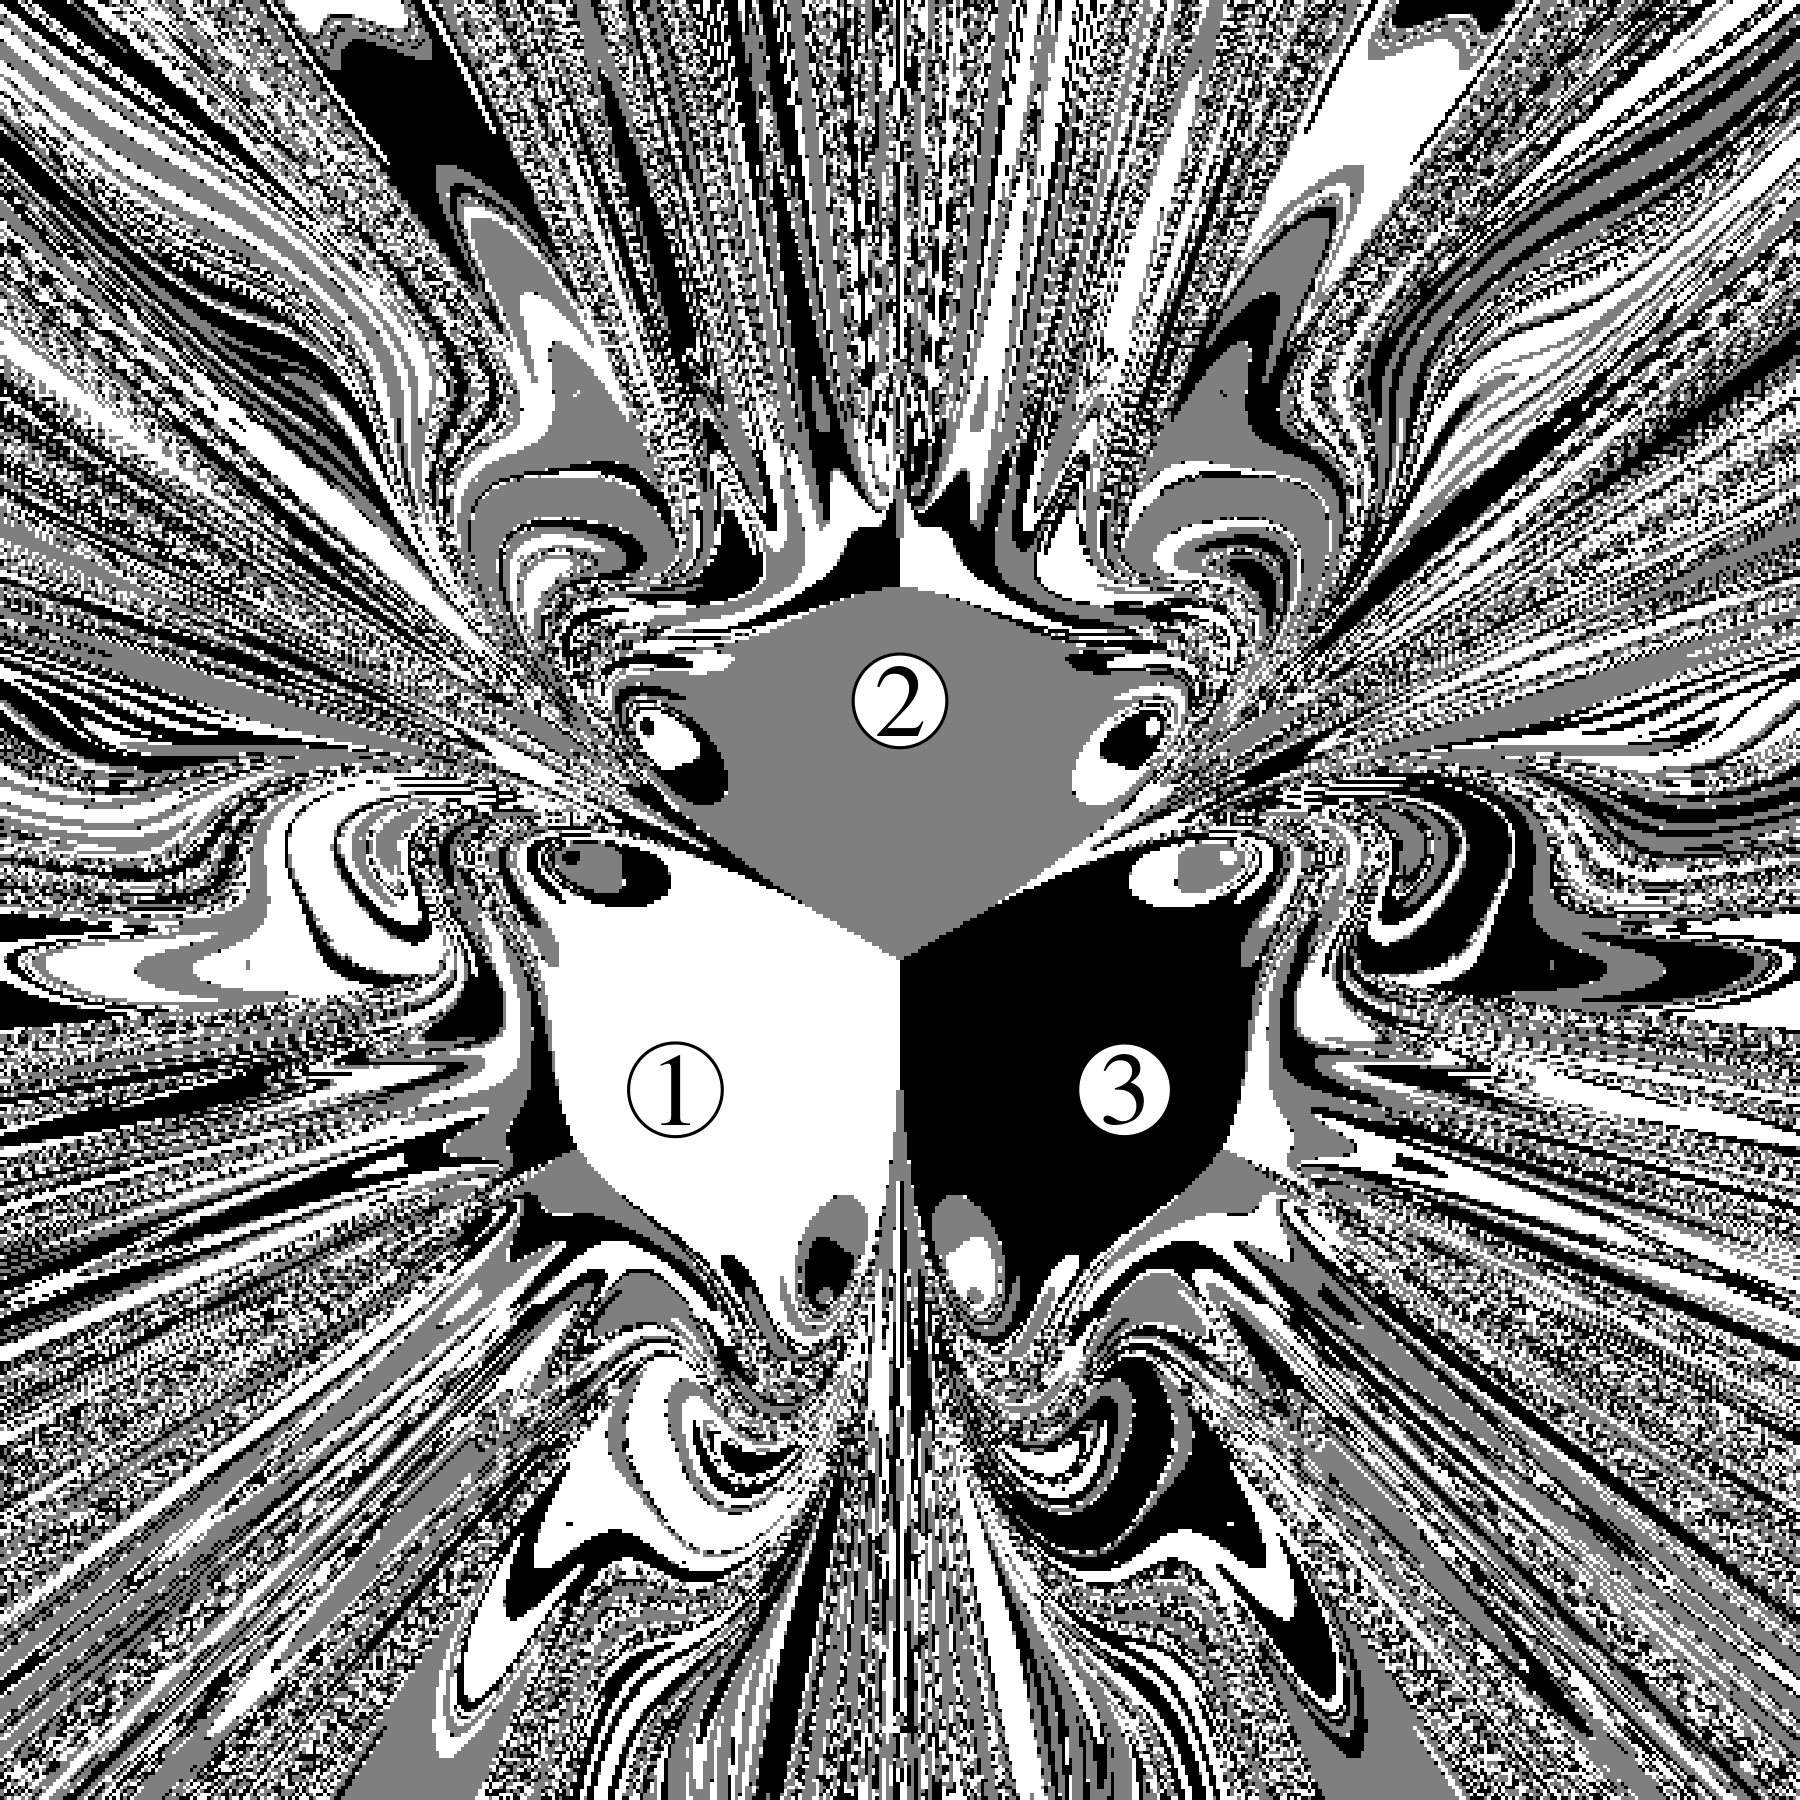
\includegraphics[width=\textwidth]{../figures/3magnets.png}\medskip
\end{minipage}
\begin{minipage}[t][][t]{.6\textwidth}
  \captionof{figure}{This intricate picture colour codes the initial
    positions of the magnetic pendulum experiment according to its
    outcomes. White, grey and black pixels in this $512\times{512}$
    image mark initial positions that resulted in a final position at
    the first, second and third magnet, respectively. The resulting
    pattern is simple in the immediate vicinity of the magnets, but
    complex at a further distance. It has all the characteristics of a
    fractal, exhibiting the same level of complexity regardless of
    scale. The pattern is determinisitic in the sense that the same
    grid of initial conditions produces exactly the same pattern. But
    it is chaotic because even tiny changes in the initial positions
    or velocity may produce completely different patterns.  }
  \label{fig:3magnets}
\end{minipage}

The strong sensitivity of the outcome on the initial conditions of the
magnetic pendulum experiments is the hallmark of \textbf{deterministic
  chaos}. It is the phenomenon whereby ``the present determines the
future, but the approximate present does not approximately determine
the future''.\medskip

The magnetic pendulum is just one example of a simple system of
\emph{coupled equations} that produces complex outcomes. It is a
geologically relevant example, because the gravitational interaction
between the planets and moons in our solar system produces similar
chaotic behaviour.  The interplay between the multitude of
gravitational fields in our solar system is responsible for the
ejection of meteors from the asteroid belt, which have been linked to
some of the largest mass extinctions in the history of
life. Gravitational interactions also destabilise the orbital
parameters of planets such as Mars. The obliquity of Mars' spin axis
is chaotic. Its evolution can be predicted thousands of years into the
future, but becomes unpredictable over million year timescales. Rapid
changes in the obliquity of Mars have caused its polar ice caps to
shift over time.\medskip

Chaos theory originates from the work of atmospheric scientist Edward
Lorenz. Lorenz formulated a simplified mathematical model for
atmospheric convection, based on three \emph{deterministic} equations.
Like the three magnets of the pendulum example, the interactions
between the three Lorenz equations produced outcomes that were
extremely sensitive to the initial conditions. Lorenz called this the
\textbf{butterfly effect}.\medskip

In the magnetic pendulum example there were just three outcomes, but
in the real world there are countless numbers of them. The butterfly
effect raises the theoretical possibility that the flap of a
butterfly's wings in Brazil may change the initial conditions of the
global atmosphere and thereby cause a tornado in Texas. Of course the
vast majority of butterfly wingflaps won't have this outcome, but some
of them may. The outcome is impossible to predict far in advance.
This phenomenon limits the ability of meteorologists to forecast the
weather more than 10 days in advance.
